\documentclass[10pt]{article}
\usepackage{latexsym}
\usepackage{natbib}
\usepackage{graphicx}
\usepackage{caption}
\usepackage{subcaption}
\usepackage{listings}

\title{Homework 2: Independent Component Analysis}
\author{Name: Shun Zhang\\
Email address: \texttt{jensen.zhang@utexas.edu}\\
EID: \texttt{sz4554}}
\date{}

\begin{document}
\maketitle

\section{Independent Component Analysis}

In this report, I applied Independent Component Analysis on Blind Source
Separation problem.

\section{Experiment}

\begin{figure}[h]
\centering
\begin{subfigure}{0.49\textwidth}
	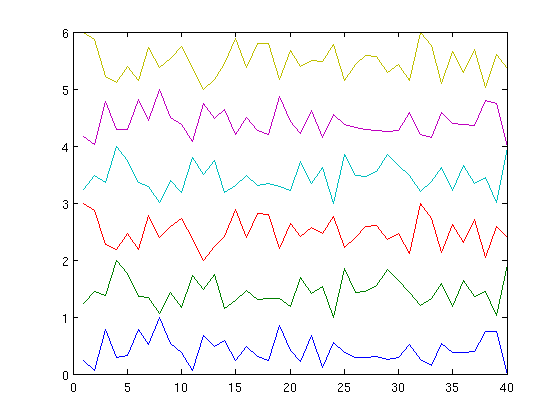
\includegraphics[width=\textwidth]{rep5.png}
\end{subfigure}
\begin{subfigure}{0.49\textwidth}
	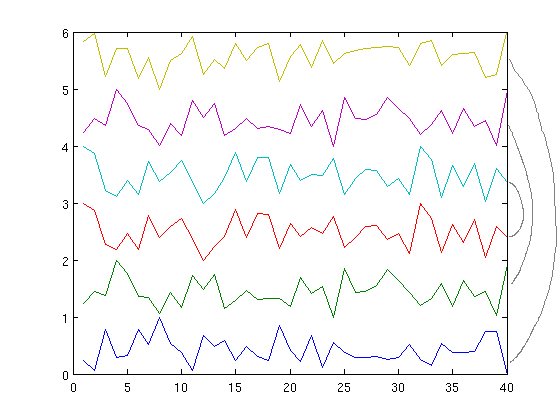
\includegraphics[width=\textwidth]{rep4.png}
\end{subfigure}
\caption{The bottom 3 lines are original signals from
\texttt{icaTest.mat}. The top 3 lines are reconstructed signals with $\eta
= 0.01$ and 1000000 iterations. Two independent experiments are shown.}
\label{fig:rep}
\end{figure}

\begin{table}
\centering
\begin{tabular}{ | l l l l | }
\hline
& Recon. 1& Recon. 2& Recon. 3\\
Source 1&-0.4900& 0.9905& -0.4248\\
Source 2&0.9918& -0.3957& -0.5454\\
Source 3&-0.4829& -0.5073& 0.9924\\
\hline
\end{tabular}
\caption{Linear correlation between source and reconstructed signals, for
the left figure in Figure~\ref{fig:rep}.}
\label{tbl:corr}
\end{table}

\begin{table}
\centering
\begin{tabular}{ | l l l l | }
\hline
& Recon. 1& Recon. 2& Recon. 3\\
Source 1 &-0.4248&-0.5454& 0.9924\\
Source 2 &-0.4900& 0.9918&-0.4829\\
Source 3 &-0.9905& 0.3957& 0.5073\\
\hline
\end{tabular}
\caption{Linear correlation between source and reconstructed signals, for
the right figure in Figure~\ref{fig:rep}.}
\end{table}

The results are scaled into $[0, 1]$ interval. This experiment is repeated
twice.  The results are in shown in Figure~\ref{fig:rep}. The result can be
permutation of the original sources. Scaling is also possible (as the
results are scaled into $[0, 1]$, the signal could be flipped in this
case). The correlation between source and reconstructed signals are shown in
Table~\ref{tbl:corr}. They are highly correlated if the correlavance is
clost to $1$ or $-1$. We can tell in the left figure, the mapping is
0-4, 1-5, 2-3. While in the right one, the mapping is 0-5, 1-3, 2-4. This
result can be verified visually.

We can observe that the constructed signal is flipped for the third source
in the right figure. It is negatively correlated with its reconstructed
signal. Also, the algorithm overall generate highly close signal, with has
more than $0.99$ correlavance with its source signal.

\begin{figure}
\centering
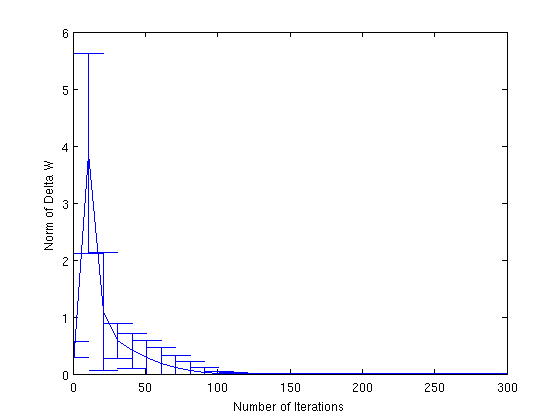
\includegraphics[width=.6\textwidth]{detW.png}
\caption{$\Delta W$ over number of iterations. Average of 5 runs. The
length of vertical bars is $\sigma$ assmuing Gaussian distribution of data
points at each iteration.}
\label{fig:detW}
\end{figure}

I also examine how progress is made in each iteration in the learning
process. As the algorithm uses gradient descent, the update on $W$ each
step, which is $\Delta W$, is useful. For the convenience of visualization,
I need the magtitude of this matrix. I use the largest singular value here,
which can be got by \texttt{norm} function when applied to a matrix.

The result is shown in Figure~\ref{fig:detW}.

Result on sound.

\section{Discussion}

\section{Conclusion}

\end{document}
